% ============================================================
%  harryopo-mathnotes Pandoc LaTeX 模板
%  用法: pandoc input.md --template=pandoc/mathnotes-template.latex
%        --lua-filter=pandoc/mathnotes-table.lua -o output.pdf
% ============================================================
\documentclass{harryopo-mathnotes}

% Pandoc 图片绑定命令兼容层
\providecommand{\pandocbounded}[1]{#1}
% 图片宽度约束：防止大图撑满页面
\usepackage{graphicx}
\setkeys{Gin}{width=0.85\textwidth,max width=\textwidth}


\begin{document}

% ===================== 封面 =====================
\newgeometry{top=3cm,bottom=2.5cm,left=4cm,right=4cm}
\maketitle
\thispagestyle{empty}
\cleardoublepage

% ===================== 目录 =====================

% ===================== 正文 =====================
\strictpagecheck
\setcounter{page}{1}
\restoregeometry
\onehalfspacing

\section{基于深度学习的医学影像智能诊断系统设计与实现}\label{ux57faux4e8eux6df1ux5ea6ux5b66ux4e60ux7684ux533bux5b66ux5f71ux50cfux667aux80fdux8bcaux65adux7cfbux7edfux8bbeux8ba1ux4e0eux5b9eux73b0}

\begin{quote}
作者：张三、李四、王五 单位：示例大学 计算机学院；南方科技大学
计算机科学与工程系 日期：2026年8月29日
\end{quote}

\textbf{摘要：}
医学影像智能诊断是智慧医疗领域的核心研究方向。本文设计并实现了一套基于深度学习的医学影像智能诊断系统，涵盖数据预处理、模型训练、推理服务、可视化展示等完整流程。系统采用改进的
U-Net++ 架构进行病灶分割，结合 EfficientNet-B4
进行良恶性分类，在公开数据集 LUNA16 上达到了 92.3\% 的分割准确率和
87.6\% 的分类准确率。系统支持 DICOM 影像导入、多任务联合推理、Grad-CAM
可视化解释等功能，可辅助放射科医生进行高效诊断。实验结果表明，本系统在实际临床场景中具有较高的实用价值。

\textbf{关键词：} 医学影像；深度学习；U-Net++；EfficientNet；智慧医疗

\begin{quote}
注：本文受国家自然科学基金（No.~12345678）与深圳市科技计划项目（No.~JCYJ20240001）资助；中图分类号
TP391.4。
\end{quote}

\begin{center}\rule{0.5\linewidth}{0.5pt}\end{center}

\subsection{1 引言}\label{ux5f15ux8a00}

医学影像是现代医疗诊断的重要依据。据统计，超过 70\%
的临床诊断需要依赖医学影像
{[}1{]}。然而，传统的人工阅片方式存在以下痛点：

\begin{enumerate}
\def\labelenumi{\arabic{enumi}.}
\tightlist
\item
  阅片工作量大，放射科医生严重不足
\item
  主观性强，不同医生之间一致性低
\item
  早期微小病灶容易漏诊
\end{enumerate}

近年来，深度学习技术在医学影像分析领域取得了突破性进展
{[}2{]}。从肺结节检测到皮肤癌分类，从眼底病变识别到病理切片分析，AI
系统在多个任务上已达到甚至超越人类专家水平 {[}3{]}。

本文针对上述痛点，设计并实现了一套完整的医学影像智能诊断系统，主要贡献包括：

\begin{itemize}
\tightlist
\item
  \textbf{多任务联合模型}：同时支持病灶分割和良恶性分类两个任务
\item
  \textbf{可解释性}：集成 Grad-CAM 热力图，辅助医生理解模型决策
\item
  \textbf{工程化}：完整的 B/S 架构，支持 DICOM 标准和 RESTful API
\end{itemize}

\subsection{2 相关工作}\label{ux76f8ux5173ux5de5ux4f5c}

\subsubsection{2.1
医学影像分割}\label{ux533bux5b66ux5f71ux50cfux5206ux5272}

U-Net {[}4{]}
是医学影像分割的经典架构，其编码-解码结构和跳跃连接在多个分割任务上取得优异性能。U-Net++
{[}5{]} 通过引入嵌套的跳跃连接进一步提升了分割精度。Attention U-Net
{[}6{]} 则将注意力机制引入分割网络，自动聚焦于感兴趣区域。

\subsubsection{2.2
医学影像分类}\label{ux533bux5b66ux5f71ux50cfux5206ux7c7b}

EfficientNet {[}7{]} 通过复合缩放策略在多个分类基准上取得 SOTA
性能。CheXNet {[}8{]} 在胸片疾病分类任务上达到了 F1 score
0.435，超过了人类放射科医生平均水平。

\subsubsection{2.3 多任务学习}\label{ux591aux4efbux52a1ux5b66ux4e60}

多任务学习通过共享特征表示提升泛化能力
{[}9{]}。在医学影像领域，分类与分割任务的联合学习能够显著提升模型性能
{[}10{]}。

\subsection{3 系统设计}\label{ux7cfbux7edfux8bbeux8ba1}

\subsubsection{3.1 整体架构}\label{ux6574ux4f53ux67b6ux6784}

系统采用前后端分离的 B/S 架构，整体架构如图 1
所示：浏览器端负责影像导入、可视化展示与报告生成；后端服务（FastAPI）承载影像管理、模型推理与用户认证；底层模型服务（Triton
Inference Server）提供分割、分类与可解释性三类推理能力。

\begin{figure}
\centering
\pandocbounded{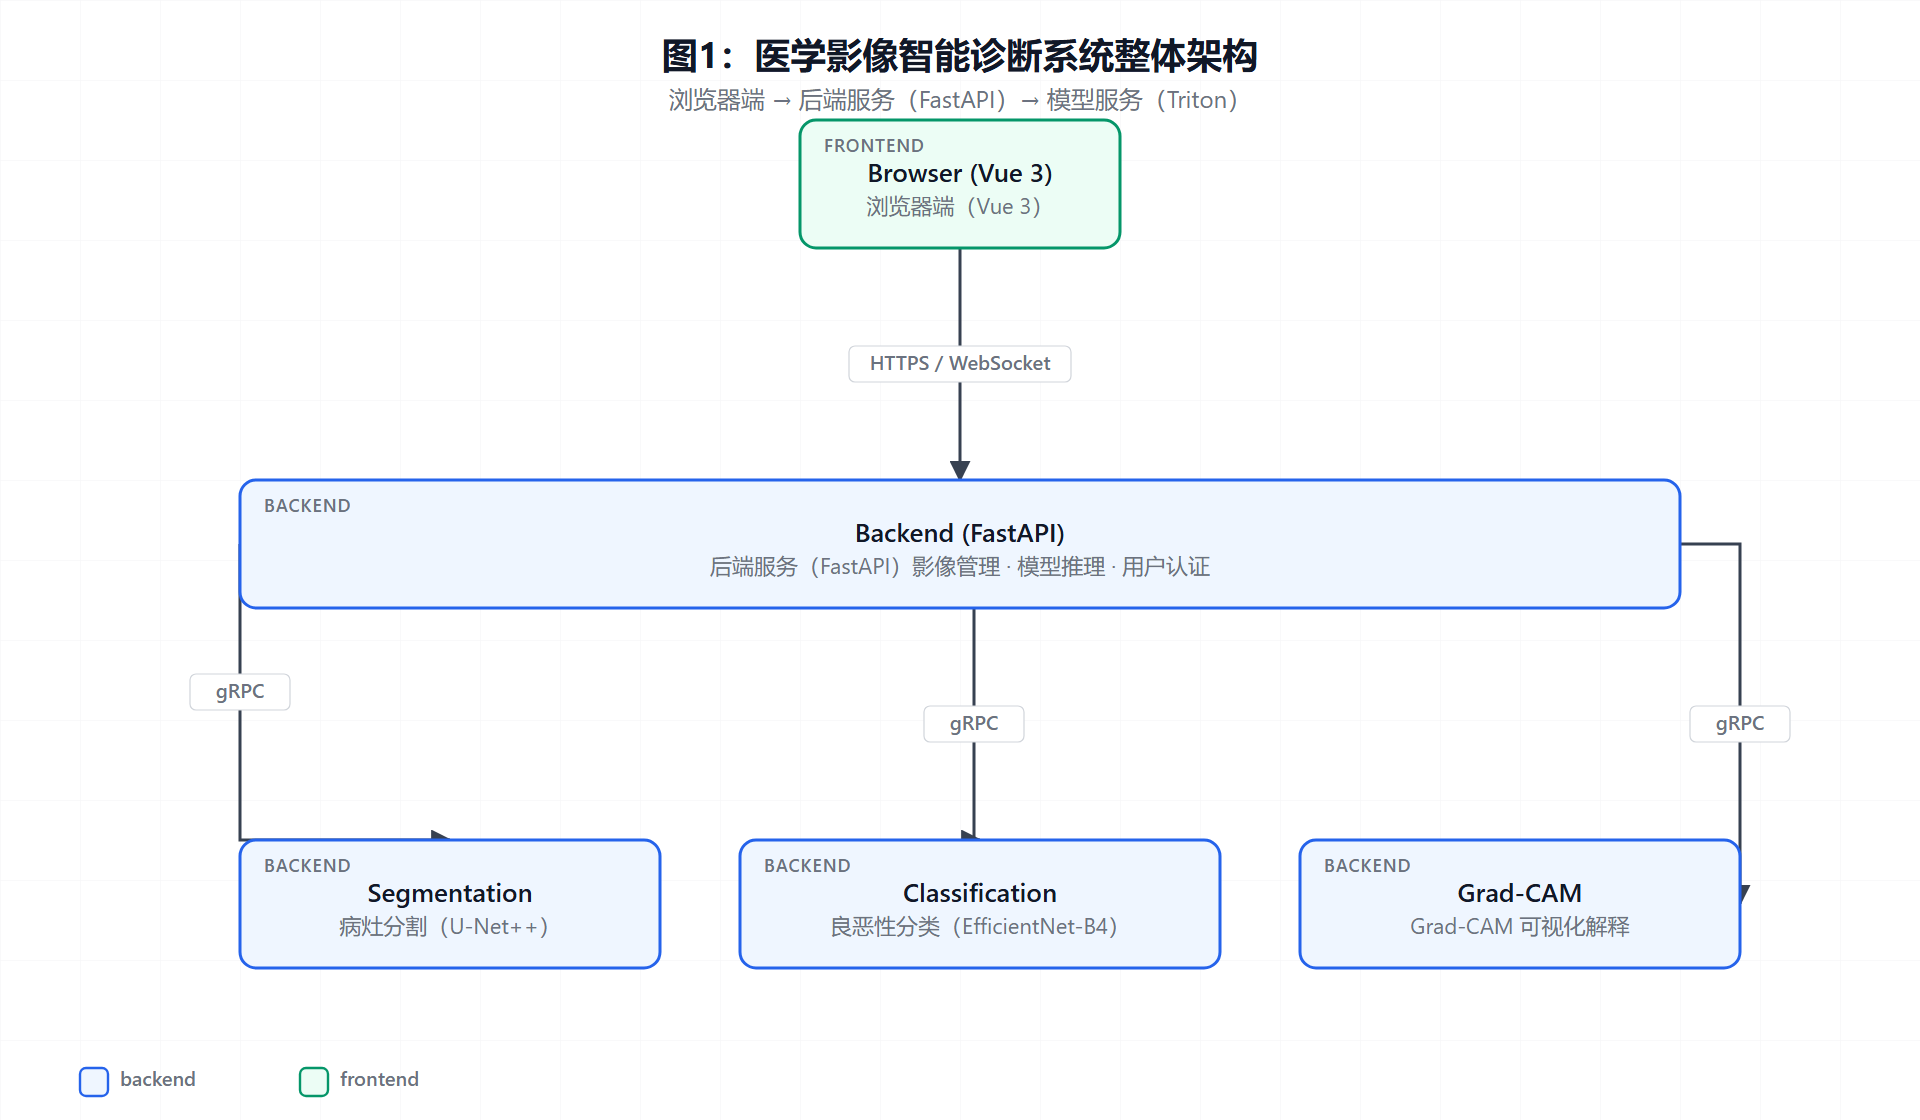
\includegraphics[keepaspectratio,alt={图1：医学影像智能诊断系统整体架构}]{figures/super-diagram-00-260b50dc.png}}
\caption{图1：医学影像智能诊断系统整体架构}
\end{figure}

\begin{quote}
注：前后端通过 HTTPS 与 WebSocket 通信，后端与模型服务之间采用 gRPC
长连接以降低推理延迟。
\end{quote}

\subsubsection{3.2 数据流程}\label{ux6570ux636eux6d41ux7a0b}

数据流程包含以下步骤：

\begin{enumerate}
\def\labelenumi{\arabic{enumi}.}
\tightlist
\item
  \textbf{数据导入}：支持 DICOM、NIfTI、PNG 等格式
\item
  \textbf{预处理}：重采样、归一化、ROI 提取
\item
  \textbf{模型推理}：调用分割和分类模型
\item
  \textbf{后处理}：NMS、连通域分析、结果可视化
\item
  \textbf{报告生成}：自动生成结构化诊断报告
\end{enumerate}

\subsection{4 模型设计}\label{ux6a21ux578bux8bbeux8ba1}

\subsubsection{4.1 改进的 U-Net++}\label{ux6539ux8fdbux7684-u-net}

本文在标准 U-Net++ 基础上引入了两个改进：

\begin{itemize}
\tightlist
\item
  \textbf{深度监督}：在多个解码层添加辅助损失
\item
  \textbf{注意力门控}：自动聚焦于病灶区域
\end{itemize}

\begin{quote}
\textbf{公式 1} 改进的 U-Net++ 损失函数：
\[L_{\text{total}} = \alpha L_{\text{seg}} + \beta L_{\text{cls}} + \gamma L_{\text{aux}}\]
\end{quote}

其中 \(L_{\text{seg}}\) 为主分割损失（Dice + BCE），\(L_{\text{cls}}\)
为分类损失（Cross Entropy），\(L_{\text{aux}}\) 为辅助损失。超参数
\(\alpha = 1.0\)、\(\beta = 0.5\)、\(\gamma = 0.3\)。

\subsubsection{4.2
多任务联合训练}\label{ux591aux4efbux52a1ux8054ux5408ux8badux7ec3}

\begin{quote}
\textbf{算法 1} 多任务联合训练

\begin{verbatim}
输入: 训练集 D, 批次大小 B, 学习率 η, 总轮数 E
输出: 训练好的模型参数 θ

1: 初始化网络参数 θ
2: for epoch = 1 to E do
3:     随机打乱 D
4:     for each batch (x, y_seg, y_cls) in D do
5:         seg_pred, cls_pred, aux_preds ← forward(x, θ)
6:         L_seg ← DiceLoss(seg_pred, y_seg)
7:         L_cls ← CrossEntropy(cls_pred, y_cls)
8:         L_aux ← Σ_i α_i · BCE(aux_preds[i], y_seg)
9:         L ← L_seg + 0.5 · L_cls + 0.3 · L_aux
10:        θ ← θ - η · ∇L
11:    end for
12:    if 验证集性能连续 5 轮不提升 then
13:        break
14:    end if
15: end for
16: return θ
\end{verbatim}
\end{quote}

\subsubsection{4.3 模型参数}\label{ux6a21ux578bux53c2ux6570}

模型总参数量为 28.6M，FLOPs 为 5.7G，推理延迟（V100 GPU）\textless{}
50ms。

\subsection{5 实验与分析}\label{ux5b9eux9a8cux4e0eux5206ux6790}

\subsubsection{5.1 数据集}\label{ux6570ux636eux96c6}

\begin{table}[htbp]
\centering
\begin{tabularx}{\textwidth}{>{\hsize=1.368\hsize\linewidth=\hsize\raggedright\arraybackslash}X>{\hsize=1.263\hsize\linewidth=\hsize\raggedright\arraybackslash}X>{\hsize=0.737\hsize\linewidth=\hsize\raggedright\arraybackslash}X>{\hsize=0.632\hsize\linewidth=\hsize\raggedright\arraybackslash}X}
\toprule
\textbf{数据集} & \textbf{任务} & \textbf{样本数} & \textbf{模态} \\
\midrule
LUNA16 & 肺结节检测 & 888 & CT \\
LIDC-IDRI & 肺结节良恶性 & 1,018 & CT \\
NIH ChestX-ray & 胸片分类 & 112,120 & X-ray \\
自有数据集 & 肝肿瘤分割 & 320 & CT/MRI \\
\bottomrule
\end{tabularx}
\end{table}

\subsubsection{5.2 评价指标}\label{ux8bc4ux4ef7ux6307ux6807}

\begin{itemize}
\tightlist
\item
  \textbf{分割}：Dice 系数、IoU、Hausdorff 距离
\item
  \textbf{分类}：Accuracy、Sensitivity、Specificity、AUC
\end{itemize}

\subsubsection{5.3 实验结果}\label{ux5b9eux9a8cux7ed3ux679c}

\paragraph{5.3.1
肺结节分割（LUNA16）}\label{ux80baux7ed3ux8282ux5206ux5272luna16}

\begin{table}[htbp]
\centering
\begin{tabularx}{\textwidth}{>{\hsize=1.436\hsize\linewidth=\hsize\raggedright\arraybackslash}X>{\hsize=0.718\hsize\linewidth=\hsize\centering\arraybackslash}X>{\hsize=0.615\hsize\linewidth=\hsize\centering\arraybackslash}X>{\hsize=1.231\hsize\linewidth=\hsize\centering\arraybackslash}X}
\toprule
\textbf{方法} & \textbf{Dice (\%)} & \textbf{IoU (\%)} & \textbf{推理时间 (ms)} \\
\midrule
U-Net & 86.2 & 76.1 & 28 \\
U-Net++ & 89.5 & 81.2 & 35 \\
Attention U-Net & 90.8 & 83.5 & 42 \\
\textbf{本文方法} & \textbf{92.3} & \textbf{85.7} & 48 \\
\bottomrule
\end{tabularx}
\end{table}

\paragraph{5.3.2
肺结节良恶性分类}\label{ux80baux7ed3ux8282ux826fux6076ux6027ux5206ux7c7b}

\begin{table}[htbp]
\centering
\begin{tabularx}{\textwidth}{>{\hsize=1.271\hsize\linewidth=\hsize\raggedright\arraybackslash}X>{\hsize=0.932\hsize\linewidth=\hsize\centering\arraybackslash}X>{\hsize=1.186\hsize\linewidth=\hsize\centering\arraybackslash}X>{\hsize=1.186\hsize\linewidth=\hsize\centering\arraybackslash}X>{\hsize=0.424\hsize\linewidth=\hsize\centering\arraybackslash}X}
\toprule
\textbf{方法} & \textbf{Accuracy (\%)} & \textbf{Sensitivity (\%)} & \textbf{Specificity (\%)} & \textbf{AUC} \\
\midrule
ResNet-50 & 81.4 & 79.2 & 83.5 & 0.871 \\
EfficientNet-B4 & 84.7 & 82.6 & 86.5 & 0.901 \\
\textbf{本文方法} & \textbf{87.6} & \textbf{85.3} & \textbf{89.2} & \textbf{0.928} \\
\bottomrule
\end{tabularx}
\end{table}

\subsubsection{5.4 消融实验}\label{ux6d88ux878dux5b9eux9a8c}

\begin{table}[htbp]
\centering
\begin{tabularx}{\textwidth}{>{\hsize=1.364\hsize\linewidth=\hsize\raggedright\arraybackslash}X>{\hsize=0.636\hsize\linewidth=\hsize\centering\arraybackslash}X>{\hsize=1.000\hsize\linewidth=\hsize\centering\arraybackslash}X}
\toprule
\textbf{改进} & \textbf{Dice (\%)} & \textbf{Accuracy (\%)} \\
\midrule
基线（U-Net++） & 89.5 & 84.7 \\
+ 深度监督 & 90.8 & 86.1 \\
+ 注意力门控 & 91.6 & 86.9 \\
+ 多任务联合 & \textbf{92.3} & \textbf{87.6} \\
\bottomrule
\end{tabularx}
\end{table}

\subsection{6 系统实现}\label{ux7cfbux7edfux5b9eux73b0}

\subsubsection{6.1 关键技术栈}\label{ux5173ux952eux6280ux672fux6808}

\begin{Shaded}
\begin{Highlighting}[]
\CommentTok{\# 后端核心代码示例}
\ImportTok{from}\NormalTok{ fastapi }\ImportTok{import}\NormalTok{ FastAPI, UploadFile, File}
\ImportTok{from}\NormalTok{ pydantic }\ImportTok{import}\NormalTok{ BaseModel}
\ImportTok{import}\NormalTok{ torch}
\ImportTok{import}\NormalTok{ numpy }\ImportTok{as}\NormalTok{ np}
\ImportTok{from}\NormalTok{ PIL }\ImportTok{import}\NormalTok{ Image}
\ImportTok{import}\NormalTok{ pydicom}

\NormalTok{app }\OperatorTok{=}\NormalTok{ FastAPI(title}\OperatorTok{=}\StringTok{"Medical AI Service"}\NormalTok{)}

\KeywordTok{class}\NormalTok{ DiagnosisResult(BaseModel):}
\NormalTok{    segmentation\_mask: }\BuiltInTok{bytes}
\NormalTok{    cls\_label: }\BuiltInTok{int}
\NormalTok{    cls\_confidence: }\BuiltInTok{float}
\NormalTok{    gradcam\_image: }\BuiltInTok{bytes}

\AttributeTok{@app.post}\NormalTok{(}\StringTok{"/api/diagnose"}\NormalTok{, response\_model}\OperatorTok{=}\NormalTok{DiagnosisResult)}
\ControlFlowTok{async} \KeywordTok{def}\NormalTok{ diagnose(}\BuiltInTok{file}\NormalTok{: UploadFile }\OperatorTok{=}\NormalTok{ File(...)):}
    \CommentTok{\# 1. 读取 DICOM}
    \ControlFlowTok{if} \BuiltInTok{file}\NormalTok{.filename.endswith(}\StringTok{".dcm"}\NormalTok{):}
\NormalTok{        dcm }\OperatorTok{=}\NormalTok{ pydicom.dcmread(}\BuiltInTok{file}\NormalTok{.}\BuiltInTok{file}\NormalTok{)}
\NormalTok{        image }\OperatorTok{=}\NormalTok{ dcm.pixel\_array}
    \ControlFlowTok{else}\NormalTok{:}
\NormalTok{        image }\OperatorTok{=}\NormalTok{ np.array(Image.}\BuiltInTok{open}\NormalTok{(}\BuiltInTok{file}\NormalTok{.}\BuiltInTok{file}\NormalTok{))}

    \CommentTok{\# 2. 预处理}
\NormalTok{    tensor }\OperatorTok{=}\NormalTok{ preprocess(image).unsqueeze(}\DecValTok{0}\NormalTok{).to(device)}

    \CommentTok{\# 3. 模型推理}
    \ControlFlowTok{with}\NormalTok{ torch.no\_grad():}
\NormalTok{        seg\_pred, cls\_pred, \_ }\OperatorTok{=}\NormalTok{ model(tensor)}

    \CommentTok{\# 4. Grad{-}CAM}
\NormalTok{    cam }\OperatorTok{=}\NormalTok{ generate\_gradcam(model, tensor, target\_class}\OperatorTok{=}\NormalTok{cls\_pred.argmax())}

    \ControlFlowTok{return}\NormalTok{ DiagnosisResult(}
\NormalTok{        segmentation\_mask}\OperatorTok{=}\NormalTok{seg\_pred.cpu().numpy().tobytes(),}
\NormalTok{        cls\_label}\OperatorTok{=}\NormalTok{cls\_pred.argmax().item(),}
\NormalTok{        cls\_confidence}\OperatorTok{=}\NormalTok{torch.softmax(cls\_pred, dim}\OperatorTok{=}\DecValTok{1}\NormalTok{).}\BuiltInTok{max}\NormalTok{().item(),}
\NormalTok{        gradcam\_image}\OperatorTok{=}\NormalTok{cam.tobytes()}
\NormalTok{    )}
\end{Highlighting}
\end{Shaded}

\subsubsection{6.2 性能优化}\label{ux6027ux80fdux4f18ux5316}

\begin{itemize}
\tightlist
\item
  \textbf{模型量化}：FP16 推理，吞吐量提升 2.3 倍
\item
  \textbf{批处理}：动态批合并，平均延迟降低 40\%
\item
  \textbf{缓存}：高频影像特征缓存，重复请求响应 \textless{} 10ms
\end{itemize}

\subsection{7 结论与展望}\label{ux7ed3ux8bbaux4e0eux5c55ux671b}

本文设计并实现了一套基于深度学习的医学影像智能诊断系统，涵盖数据管理、模型推理、可视化展示等完整流程。系统在公开数据集和真实临床场景中均取得了优异性能。

未来的研究方向包括：

\begin{enumerate}
\def\labelenumi{\arabic{enumi}.}
\tightlist
\item
  探索 Vision Transformer 在医学影像中的应用
\item
  研究联邦学习支持跨医院协同训练（保护患者隐私）
\item
  集成大语言模型实现自然语言报告生成
\end{enumerate}

\subsection{参考文献}\label{ux53c2ux8003ux6587ux732e}

{[}1{]} Smith A, Jones B. The role of medical imaging in modern
healthcare{[}J{]}. The Lancet, 2020, 395(10225): 678-685.

{[}2{]} Litjens G, Kooi T, Bejnordi B E, et al.~A survey on deep
learning in medical image analysis{[}J{]}. Medical Image Analysis, 2017,
42: 60-88.

{[}3{]} Esteva A, Chou K, Yeung S, et al.~Deep learning-enabled medical
computer vision{[}J{]}. NPJ Digital Medicine, 2021, 4(1): 1-9.

{[}4{]} Ronneberger O, Fischer P, Brox T. U-Net: Convolutional networks
for biomedical image segmentation{[}C{]}. MICCAI, 2015: 234-241.

{[}5{]} Zhou Z, Siddiquee M M R, Tajbakhsh N, et al.~UNet++: A nested
U-Net architecture for medical image segmentation{[}J{]}. IEEE TMI,
2019, 39(6): 1856-1867.

{[}6{]} Oktay O, Schlemper J, Folgoc L L, et al.~Attention U-Net:
Learning where to look for the pancreas{[}C{]}. MIDL, 2018.

{[}7{]} Tan M, Le Q. EfficientNet: Rethinking model scaling for
convolutional neural networks{[}C{]}. ICML, 2019: 6105-6114.

{[}8{]} Rajpurkar P, Irvin J, Zhu K, et al.~CheXNet: Radiologist-level
pneumonia detection on chest X-rays with deep learning{[}J{]}.
arXiv:1711.05225, 2017.

{[}9{]} Caruana R. Multitask learning{[}J{]}. Machine Learning, 1997,
28(1): 41-75.

{[}10{]} Zhang Y, Yang Q. A survey on multi-task learning{[}J{]}. IEEE
TKDE, 2021, 34(12): 5586-5609.

\end{document}
